\section{Main results}
\begin{figure}
\centering
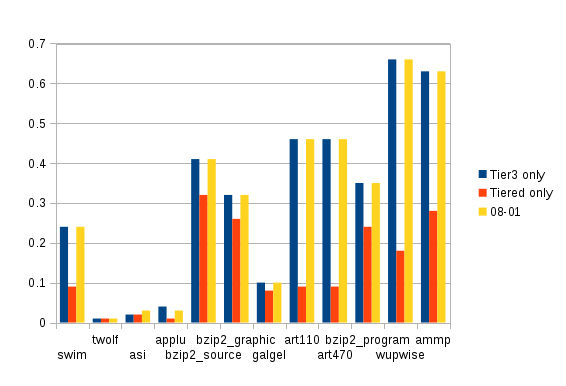
\includegraphics[width=0.55\textwidth]{images/dmarkchart.png}
\caption{The coverage of the different tests}
\label{fig:chart}
\end{figure}
No real difference was found between the various trigger values for switching modes,
but this is not surprising when considering that the prefetcher seems to have results
comparable to DCPT to a higher degree than to TDCPT, thus seemingly preferring to stay
in T3-only-mode. The miniscule gains were the same at any of the thresholds that were
attempted, so no clear conclusion was drawn as to the best threshold.

\subsection{Discussion}
Due to problems with getting the simulation to run in a stable fashion, that
were finally found to stem from some faulty memory management on our part, a
thorough set of tests was not possible to produce. The limited set of tests
that were run did however show very negligible difference.

From testing the algorithm in a purely Tiered mode, we notice that the
space that is used for the T1-table can be used more effectively as a T3
table in general, however, there seems to be some smaller cases where dynamically
switching between tiered and non-tiered mode yields a tiny advantage in coverage
over the original DCPT algorithm (as can be seen in figure \ref{fig:chart}). 
This is a fractional gain for the rather
large increase in complexity that is required to support dynamically changing how
the storage space required is used.


\subsection{Conclusion}
As there are no clear difference in the results of the DTDCPT from the ordinary
DCPT algorithm, there are no clear conclusion to be made. The tendency seems to
be of the algorithm to run as DCPT, as the speedup seen is nearly identical to
that of DCPT. The DTDCPT algorithm is thus not significantly worse than DCPT, and for other
tests than the test sets used, it might still yield a tiny improvement, albeit at the cost
of a lot more complexity to the DCPT algorithm. Since DTDCPT algorithm has a tendency towards
being similar to DCPT, but not to purely tiered in it's results, this should mean that it also
tends towards running in T3-only mode, rather than in Tiered-mode. Thus we can conclude that either
our limited testing of limits for switching modes is faulty, or tiering has no real gain, and in most
cases is counter productive. Considering the results of Sømåen et al's results, it isn't too far fetched
to consider the latter as the more likely reasoning.

\subsection{Future Work}
The tests run did not show any usefull benefit to attempting a dynamically switching
between statically defined tier-sizes with a single tier. Further looking into dynamically
resizing the buffer to a selection of different variable sizes might better suit the varying
access patterns, and could be a possible idea for further looking into the possibilites of tiering.
A current weakness of both this attempt at looking into tiering the DCPT-entries, as well as Sømåen
et. al's attempt, is that tiering may have the possibility of keeping stale elements for a longer period,
so looking into whether this is responsible for it's rather low effectiveness might also be interesting.

Looking into even smaller memory footprints than what was tested in this paper might also be intereesting,
as when the memory footprints go down, the chance of flushing out interesting items from a T3-buffer might
perhaps increase a bit more, as Figure 13 in Grannæs et al suggests that there is a rather steep increase in
speedup between 20 and 30 entries.
